\documentclass[
  11pt,
  twocolumn,
  a4paper,
%  bibliography=totoc,     % Literatur im Inhaltsverzeichnis
]{article}


% Paket float verbessern
\usepackage{scrhack}

% Warnung, falls nochmal kompiliert werden muss
\usepackage[aux]{rerunfilecheck}

% unverzichtbare Mathe-Befehle
\usepackage{amsmath}
% viele Mathe-Symbole
\usepackage{amssymb}
% Erweiterungen für amsmath
\usepackage{mathtools}
% Fonteinstellungen
\usepackage{fontspec}
% Latin Modern Fonts werden automatisch geladen
% Alternativ zum Beispiel:
%\setromanfont{Libertinus Serif}
%\setsansfont{Libertinus Sans}
%\setmonofont{Libertinus Mono}

% Wenn man andere Schriftarten gesetzt hat,
% sollte man das Seiten-Layout neu berechnen lassen
% \recalctypearea{}
% deutsche Spracheinstellungen
\usepackage{polyglossia}
\setmainlanguage{german}

\usepackage{marvosym}
\usepackage[
  math-style=ISO,    % ┐
  bold-style=ISO,    % │
  sans-style=italic, % │ ISO-Standard folgen
  nabla=upright,     % │
  partial=upright,   % ┘
  warnings-off={           % ┐
    mathtools-colon,       % │ unnötige Warnungen ausschalten
    mathtools-overbracket, % │
  },                       % ┘
]{unicode-math}

% traditionelle Fonts für Mathematik
\setmathfont{Latin Modern Math}
% Alternativ zum Beispiel:
%\setmathfont{Libertinus Math}

\setmathfont{XITS Math}[range={scr, bfscr}]
\setmathfont{XITS Math}[range={cal, bfcal}, StylisticSet=1]

% Zahlen und Einheiten
\usepackage[
  locale=DE,                   % deutsche Einstellungen
  separate-uncertainty=true,   % immer Fehler mit \pm
  per-mode=symbol-or-fraction,
  alsoload=hep,                % / in inline math, fraction in display math
]{siunitx}
\sisetup{math-micro=\text{µ},text-micro=µ}
\DeclareSIUnit\micron{\micro\metre}
\DeclareSIUnit\mrad{\milli\rad}
\DeclareSIUnit\gauss{G}
\DeclareSIUnit\eVperc{\eV\per\clight}
\DeclareSIUnit\nanobarn{\nano\barn}
\DeclareSIUnit\picobarn{\pico\barn}
\DeclareSIUnit\femtobarn{\femto\barn}
\DeclareSIUnit\attobarn{\atto\barn}
\DeclareSIUnit\zeptobarn{\zepto\barn}
\DeclareSIUnit\yoctobarn{\yocto\barn}
\DeclareSIUnit\nb{\nano\barn}
\DeclareSIUnit\pb{\pico\barn}
\DeclareSIUnit\fb{\femto\barn}
\DeclareSIUnit\ab{\atto\barn}
\DeclareSIUnit\zb{\zepto\barn}
\DeclareSIUnit\yb{\yocto\barn}

% chemische Formeln
\usepackage[
  version=4,
  math-greek=default, % ┐ mit unicode-math zusammenarbeiten
  text-greek=default, % ┘
]{mhchem}

% richtige Anführungszeichen
\usepackage[autostyle]{csquotes}

% schöne Brüche im Text
\usepackage{xfrac}

% Standardplatzierung für Floats einstellen
\usepackage{float}
\floatplacement{figure}{htbp}
\floatplacement{table}{htbp}

\RequirePackage{luatex85}
\usepackage[
  locale=DE,
]{siunitx}

\usepackage{tikz}
\usepackage[
  europeanresistors, % follow DIN
  americaninductors, % follow DIN
  siunitx,
]{circuitikz}
\usepackage{stackengine}
\AtBeginDocument{
  \sisetup{
    math-rm=\mathrm,
    math-micro=µ, % AltGr+m = MICRO SIGN, Unicode: U+00B5
  }
}

% Floats innerhalb einer Section halten
\usepackage[
  section, % Floats innerhalb der Section halten
  below,   % unterhalb der Section aber auf der selben Seite ist ok
]{placeins}

% Seite drehen für breite Tabellen: landscape Umgebung
\usepackage{pdflscape}

% Captions schöner machen.
\usepackage[
  labelfont=bf,        % Tabelle x: Abbildung y: ist jetzt fett
  font=small,          % Schrift etwas kleiner als Dokument
  width=0.9\textwidth, % maximale Breite einer Caption schmaler
]{caption}
% subfigure, subtable, subref
\usepackage{subcaption}

% Grafiken können eingebunden werden
\usepackage{graphicx}
% größere Variation von Dateinamen möglich
\usepackage{grffile}

% schöne Tabellen
\usepackage{booktabs}

% Verbesserungen am Schriftbild
\usepackage{microtype}

% Literaturverzeichnis
\usepackage[
  backend=biber,
]{biblatex}
% Quellendatenbank
\addbibresource{lit.bib}
\addbibresource{programme.bib}

% Hyperlinks im Dokument
\usepackage[
  unicode,        % Unicode in PDF-Attributen erlauben
  pdfusetitle,    % Titel, Autoren und Datum als PDF-Attribute
  pdfcreator={},  % ┐ PDF-Attribute säubern
  pdfproducer={}, % ┘
]{hyperref}
% erweiterte Bookmarks im PDF
\usepackage{bookmark}

% Trennung von Wörtern mit Strichen
\usepackage[shortcuts]{extdash}

%Multirow Einbindung
\usepackage{multirow}

%rotating Einbindung
\usepackage{rotating}

%noindent immer da


% \documentclass[11pt, twocolumn, a4paper]{article}

\setlength{\oddsidemargin}{0.0 cm}
\setlength{\evensidemargin}{0.0 cm}
\setlength{\topmargin}{-1cm}
\setlength{\textheight}{24 cm}
\setlength{\textwidth}{16 cm}

\pagestyle{plain}

\setlength{\parindent}{0in}

\begin{document}

\author{Nils Breer}
\date{Technische Universit\"at Dortmund}

\title{Proceeding to the LHC seminar talk \textit{Update of the $B^0$ \to $K^{*0}$ µ$^{+}$ µ$^{-}$ angular analysis at LHCb experiment} held by Eluned Smith on behalf of the LHC collaboration on 13th of March 2020.}

\maketitle

% hier kommt ein abstract rein!!
(das ist von fabian! nur als hilfe benutzen um zu wissen was da so rein kann.)
The search for physics beyond the standard model continues especially in high precision measurements. One of the most promising decay types for new possible interactions are flavor changing neutral currents. In this analysis data from 2011, 2012 and 2016 is used to update the prior angular analysis of the process stated above which only used the 20111 and 2012 data. With twice the statistics and a better understanding of theoretical uncertainties the analysis confirms the local tension in $P_5\prime$ found in the first analysis. A possible explanation of the tension is given by introducing a shift to the Wilson coefficient $C_9$. This increases the significance of the tension to $2.7$ - $3.3\sigma$.

The stated Process is of such importance because the
$b \to s \mu \mu$ transition is forbidden at tree level due to FCNC and can only occur at loop order.
Because of that, these processes are much more sensitive to new physics(NP).

\begin{figure}[htb]
  \centering
  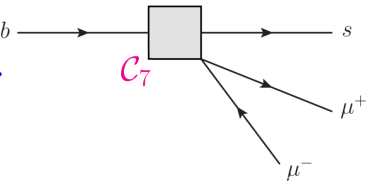
\includegraphics[width=0.5\textwidth]{flavor_plots/wilson_c7.png}
  \caption{Wilson coefficient $C_7$ in .}
  \label{fig:sm_process}
\end{figure}

\begin{figure}[htb]
  \centering
  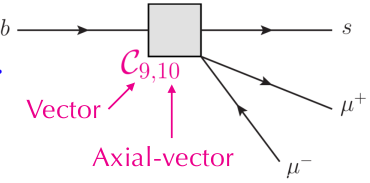
\includegraphics[width=0.5\textwidth]{flavor_plots/wilson_c9_c10.png}
  \caption{Process in new physics model.}
  \label{fig:np_process}
\end{figure}

To gather information about short distance NP above the SM energy scale $\mu$, wilson coefficients $C_i(\mu)$ and low-energy QCD Operators $O_i$ are used to describe that.

The wilson coefficients $C_7$, $C_9$ and $C_{10}$ are of great importance since observables like the forward-backward asymmetry and $P_5\prime$ are sensitive for $C_9$ especially.

In an effective theory, $C_9$ and $C_{10}$ are used to describe the contribution from loops, in which electroweak gauge bosons are produced.  wilson coefficient $C_7$ describes the contribution from loopdiagramms which produce photons from the loops.

This can be summarized by an effective hamiltonian
\begin{equation*}
  H_{eff} = - \frac{4 G_f}{\sqrt{2}} \symup{V}_{tb} \symup{V}_{ts}^{*} \sum_i
  C_i \cdot O_i + \text{h.c.}
\end{equation*}

$G_F$ is Fermi's constant, $\mu$ ist the renormalization scale, $\symup{V}_{tb} \symup{V}_ts^{*}$ is the contains leading flavor factors of the SM which lie in the CKM matrix elements $V_{ij}$

% \section{angular Analysis}
To measure the decay rate as a function of angles of the decay products, an angular analysis is performed.
This is motivated by the fact, that the $K^{0*}$ is a meson with spin 1 therefore three polarisation states. This results in a rich angular structure.
The definition of the angular observables $\theta_{k}$, $\theta_{l}$ and $\phi$ is schematically shown in figure \ref{fig:angle_1}

\begin{figure}[htb]
  \centering
  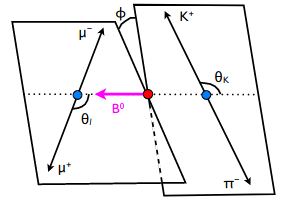
\includegraphics[width=0.5\textwidth]{flavor_plots/angular_describtion.png}
  \caption{image of the angular observables.\cite{Chatrchyan:2013cda}}
  \label{fig:angle_1}
\end{figure}

In this analysis, the forward-backard asymmetry $A_{FB}$, $F_L$ the fraction of the longitudinal polarisation of the $K^{*0}$ and the decay rate of the process $B^0 \to K^{*0} \mu \mu$ was measured. The definition of the angular observables are the following.
$\theta_{l}$ is the angle between the negatively charged lepton and  $\bar{B}$ in the dimuon center of mass system (c.m.s).
$\theta_{k}$ is the angle between the Kaon and the $\bar{B}$ in the $K^{*0}$ c.m.s..
The angle between the $K^{*0}$-plane and the dimuon-plane is defined by the angle $\phi$\cite{Bobeth:2010wg}.

Considering that S-wave contribution, spinless $K^{+}\pi^{-}$ constellations, can pollute the measurement, therfore a parametrization such as $\left(1 - F_S\right)$ for this was taken into account where $(1 -F_S)$ is the S-wave fraction which describes the amount of S-wave contribution.
The interference Amplitude between P-wave and S-wave decays are parametrized by $A_S$.
The angular distribution\cite{Chatrchyan:2013cda} for the $B^0 \to K^{*0} \mu \mu$ decay reads
\begin{equation*}
  \frac{1}{\Gamma}\frac{\symup{d}^3\Gamma}{\symup{d}\theta_k\symup{d}\theta_l\symup{d}q^2} = \frac{9}{16}f\left(F_S, A_S, \theta_k, \theta_l, A_{FB}, F_L\right)
\end{equation*}
Since $A_{FB}$, $F_L$ and $\mathcal{A}\times\Epsilon$ do not depend on the angle $\phi$, it is already integrated out.
The angular description for The $B$ and $\bar{B}$ are combined afterwards and expanded into a sum of the angular variables multiplied with a fitparameter, which are the $A_{FB}$, $F_L$ and $S_i$\ref{fig:dubgamma}, which are called CP-averaged observables because they contain CP violation.

\begin{figure}[htb]
  \centering
  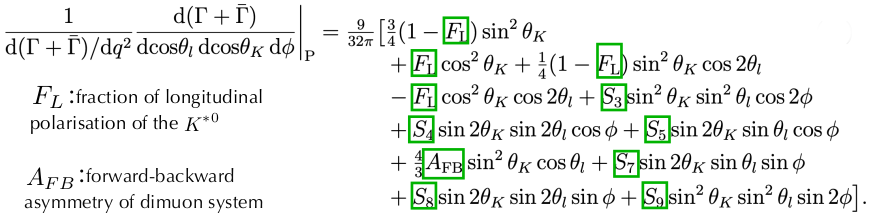
\includegraphics[width=0.5\textwidth]{flavor_plots/double_gamma.png}
  \caption{Angular description for $B$ and $\bar{B}$ combined.}
  \label{fig:dubgamma}
\end{figure}

Then the fit in the $S_i$ basis was reparametrised to the $P_i$ basis.
This was done to eliminate first order uncertainties in the form factors primarily.
The fit to the angular distribution yields seven CP violating observables including $F_L$.
The $P_i$ basis contains the amplitudes of the $K^{0*}$ as angular coefficients as seen in table \ref{tab:coefff}.
\begin{align*}
  P_1 &= \frac{2 S_3}{1 - F_L} & P_{4,5,8}\prime &= \frac{S_{4,5,8}}{\sqrt{F_L\left( 1 - F_L \right)}} \\
  P_2 &= \frac{2}{3}\frac{A_{FB}}{1 - F_L} &  P_6\prime &= \frac{S_7}{\sqrt{F_L\left( 1 - F_L \right)}} \\
  P_3 &= \frac{- S_9}{1 - F_L} \\
\end{align*}

The angular distribution can be reduced to
\begin{equation*}
  \frac{1}{\Gamma}\frac{\symup{d}^3\Gamma[\bar{B}^0 \to \bar{K}^{0*} \mu^{+} \mu^{-}]}
  {\symup{d}\cos\theta_l\symup{d}\cos\theta_k\symup{d}q^2} =
  \frac{9}{16}\sum_i S_i(q_{min}^2, q_{max}^2) f_i(\vec{\Omega})
\end{equation*}
in the $S_i$ basis.
The $S_i$ basis contains the six angular coefficients which are the combinations of the $K^{0*}$ amplitudes and $\vec{\Omega} = (\cos\theta_l, \cos\theta_k)$. These amplitudes describe the polarization states of the Kaon.

This analysis especially focuses heavily on the tension induced by $P_5\prime$, since it is a very sensitive variable for $C_9$.
This can be seen in the range of $4$ - $8$ $\frac{\symup{GeV}^2}{c^4}$ displayed in figure \ref{p5tension}.
The discrepancy is $2.8\sigma$ for the $q^2$ intervall from $4$ - $6$ $\frac{\symup{GeV}^2}{c^4}$ and $3\sigma$ for the $6$ - $8$ $\frac{\symup{GeV}^2}{c^4}$ intervall.
For every collaboration a discrepancy between the SM and the measurement
is visible, but the CMS measurement is the closest the the SM prediction.

\begin{figure}[htb]
  \centering
  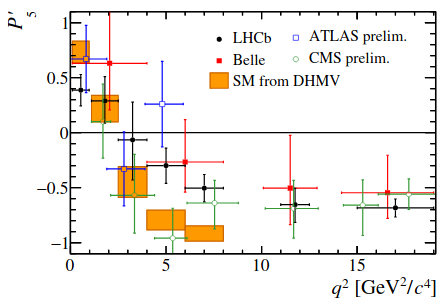
\includegraphics[width=0.5\textwidth]{flavor_plots/tension_in_p5.png}
  \caption{tension in $P_5\prime$.\cite{Blake:2017wjz}}
  \label{p5tension}
\end{figure}

For this analysis the data sets used are from the years 2011, 2012 and 2016. The data sets from 2011 and 2012 are from run 1.
The 2011 data was taken at a centre of mass energy of $\sqrt{s} = \SI{7}{\tera\electronvolt}$, the 2012 data at $\sqrt{s} = \SI{8}{\tera\electronvolt}$ and the added data set from 2016 was taken at $\sqrt{s} = \SI{13}{\tera\electronvolt}$. Adding the 2016 data also doubled the statistic to around $\SI{4.7}{\per\femto\barn}$.

For the selection of candidates it is required, that the impact paramters for the daughter particles are quite significant since they do not originate from the primary vertex.
Daughter particles that come from the primary need to have a very small impact parameter and also a quality vertex is necessary. That means the track fit $\frac{\chi^2}{dof}$ must be small, where dof are the degrees of freedom.
To suppress peaking background as seen in figure \ref{fig:q2_spec} the particle identification is used.
The FCNC process here is described by $B^0 \to K^{0*}\mu\mu$, but the subprocesses such as $B^0 \to K^{0*}\left(\bar{c}c \to \gamma^{*} \to \mu\mu\right)$ are statistical relevant since they proceed at tree level.
Therefore charmonium resonances pollute the $q^2$ spectrum, especially ate the $\symup{J}/\Psi(1S)$ and the $\phi(2S)$ mass.
Around these peaks a mass-veto region is defined where signal decays cannot occur.
Left, in between and on the right of the peaks the signal regions are defined.
A multivariate analysis(MVA) is performed to suppress combinatorial background even further.
MVA's is a machine learning technique in which a classifier or regressor takes several features to learn from and to make a prediction on what is background and what belongs to the signal.
To suppress $J/\Psi \to ll$ contributions, the invariant mass spectrum is looked at.
The most common features are: small momentum particles and small opening angles and a large $\symup{d}E / \symup{d}x$.
Since the detector cannot know which lepton pairs belong together, all possible combinations are tested. Combinations with same signed leptons ($N^{++}$ or $N^{--}$) are always uncorrelated so the signal S results in $S = N^{+-} - (N^{++} or N^{--})$. This is called the like-sign method\cite{combinatoric}.
$N^{+-}$ are the opposite sign lepton pairs.

\begin{figure}[htb]
  \centering
  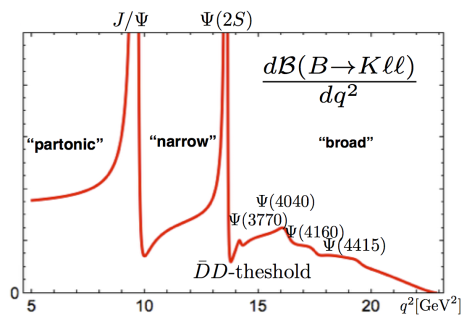
\includegraphics[width=0.5\textwidth]{flavor_plots/q2_spectrum.png}
  \caption{spectrum in $q^2$ for the \\
  lepton pair in Kll branching fraction\cite{Blake:2017wjz}.}
  \label{fig:q2_spec}
\end{figure}

Now for the full fit model the shape of the invariant mass plots are used to determine the amount of signal and background in the data.
\begin{equation*}
  \symup{PDF}_{total} = f_{sig}\symup{PDF}_{sig}(\vec{\Omega}, m) +
  (1 - f_{sig})\symup{PDF}_{bkg}(\vec{\Omega}, m)
\end{equation*}

The PDF function can be separated into an angular part and a massive part.
After that a maximum likelihood fit is performed.
As seen in figure \ref{fig:fullfit} the massive part of the signal PDF is a gaussian fucntion with a radiative tail and the background PDF results in an exponential function.

\begin{figure}[htb]
  \centering
  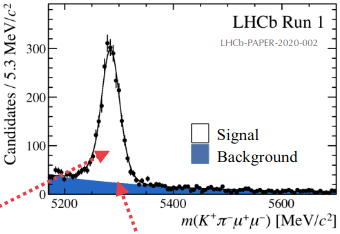
\includegraphics[width=0.5\textwidth]{pictures/fullfit.png}
  \caption{invariant B mass of Run 1 LHCb data.}
  \label{fig:fullfit}
\end{figure}

Because of the factorization of the signal and background PDF
\begin{align*}
  \symup{PDF}_{sig}(\vec{\Omega}, m) &= \symup{PDF}_{sig}(\vec{\Omega}) \times \symup{PDF}_{sig}(m) \\
  \symup{PDF}_{bkg}(\vec{\Omega}, m) &= \symup{PDF}_{bkg}(\vec{\Omega}) \times \symup{PDF}_{bkg}(m)
\end{align*}
the angular part of the signal PDF of the Run 1 data and the data from 2016 are shared in the analysis to perform a simultaneous fit $\sum_i S_{i, q_{bin}^2} f_i(\Omega)$ because the angular part of the signal PDF corresponds to $f_i(\Omega)$. The $S_i$ are thus used as fitparameters.

% % \section{modelling the efficiencies}
% Because the angular distribution and the $q^2$ distribution are influenced by the efficiencies, the parametrisation must be well known.
% This is done via an acceptance function, her the legendre polynomials. With 3 angles and $q^2$ a 4D parametrisation results in 4 coefficents
%
% % \section{s-wave contribution}
% The $K \pi$ final state has more than one spin eigenstate. Therefore, additional terms are needed to differentiate between these states.
% Because $K \pi \mu \mu$ can be produced in a vector state which disturbs the angular distribution, the different structures of the spin 1 $K^{0*}$ and the flat structure of the $K \pi$ state need to be analyzed.
%
% % \section{uncertainties}
% The dominant systematic uncertainties across the $q^2$ bins are acceptance variation with $q^2$, peaking backgrounds and the bias correction.
% The whole table of uncertainties is shown in figure \ref{fig:unc}\cite{cern}.
% \begin{figure}[htb]
%   \centering
%   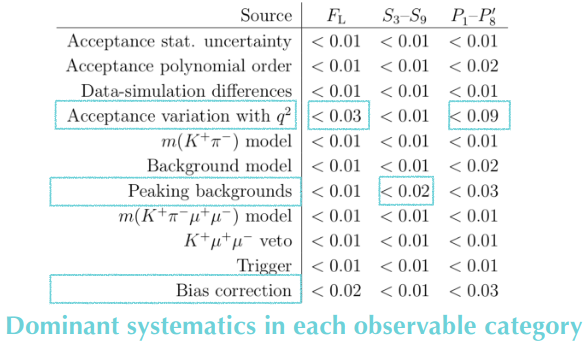
\includegraphics[width=0.5\textwidth]{pictures/uncertainties.png}
%   \caption{table of systematic uncertainties.}
%   \label{fig:unc}
% \end{figure}
%
% Because of different decays in the same target finalstate, for example $\bar{\Lambda}_b^0 \to \bar{p} \to \pi^{-} K^{+} \mu \mu$, events that are drawn from distributions of these peaking backgrounds are not taken into the fit.
% Bias corrections come up if boundary effects like $F_S > 0$ are required.
% \begin{equation*}
%   ~\frac{\symup{d}\Gamma}{\symup{d}q^2}\rvert_{S + P} = \left(1 - F_S \right) ~\frac{\symup{d}\Gamma}{\symup{d}q^2}\rvert_P
% \end{equation*}
% For small $F_S$ the bias towards higher values biases the P-wave and vice versa.
%
% % \section{Results and conclusion}
% If the energy threshold is so big, that a $c\bar{c}$ pair can be produced in a loop which generates a $J \/ \Psi$, the would be a possibility to detect it.
%
% The tension is confirmed with the 2016 data set.
% The significance of the discrepancy is nuisance parameter dependend and also depends on the $q^2$ bins.
\printbibliography{}
\end{document}
